% !TEX root = sample.tex
%%==========================================================================
\section{SuperMatching}
\label{sec:supersymhopm}
%-------------------------------------------------------------------------
We first discuss the former two issues mentioned above, which are independent of application; later we turn to definition of affinity measure, which is application dependent, and sampling strategy.


\subsection{Supersymmetric Affinity Tensor}
\label{subsec:supersymtensor}

A tensor generalizes vectors and matrices to higher dimensions: a vector is a tensor of order one,
and a matrix is a tensor of order two. A higher-order tensor can be expressed as a multi-dimensional array~\cite{Kolda08}.
Here we consider a higher-order supersymmetric affinity tensor, which represents a real-valued higher-order affinity between feature tuples.
The main motivation of using supersymmetry is try to utilize its advantage to remove the redundancy of the tensor elements, 
and the following deduction would prove that the motivation is effective.
%%%RRM One problem. You have not exaplined anywhere yet WHY the affinity
%%%RRM tensor should be supersymmetric. This is an important issue which needs
%%%RRM to come here.
%%Done

\newtheorem{mot}{Definition}
\begin{mot}[Supersymmetric Tensor]
\label{mot:def1}
A tensor is  \emph{supersymmetric} if its entries are invariant under any permutation of its indices~\cite{Kofidis02}.
\end{mot}

For example, a third-order supersymmetric tensor $\mathcal{T}_3$, satisfies the relationships:
$\mathcal{T}_3(i_1, i_2, i_3)=\mathcal{T}_3(i_1, i_3, i_2)=\mathcal{T}_3(i_2, i_1, i_3)=\mathcal{T}_3(i_2, i_3, i_1)=\mathcal{T}_3(i_3, i_1, i_2)=\mathcal{T}_3(i_3, i_2, i_1)$.

\begin{mot}[Supersymmetric Affinity Tensor]
\label{mot:def2}
Given two feature sets $P$ and $Q$, with $N_1$ and $N_2$ features respectively,
the supersymmetric affinity tensor is an $N^{th}$ order $I_1\cdots \times I_N$, nonnegative tensor $\mathcal{T_N}$,
where $I_1, \cdots ,I_N=N_1N_2$, for which there exists a set of indices $\theta_N$,
and an $N^{th}$ order potential function $\phi_N$, such that
%
\begin{flalign}
\mathcal{T}_N(i_1,\ldots,i_N) = \begin{cases}
\phi_N(\Omega(i_1,\ldots,i_N))&{,\forall(i_1,\ldots,i_N)\in \theta_N}  \\
\quad{}\quad{}\quad{}   0     &{,\forall(i_1,\ldots,i_N)\notin \theta_N}
\end{cases}
\end{flalign}
%
where $\Omega$ stands for an arbitrary permutation of the vector, and $\theta_N$ satisfies $\forall (i_1,\ldots,i_N)\in \theta_N, \forall i_m\in\{i_1, \ldots, i_N\}$
and $\forall i_n\in\{i_1, \ldots, i_N\}-\{i_m\}$ meets the requirement that $i_m \neq i_n$.
\end{mot}

A tensor element with $(i_1,\ldots,i_N)\in \theta_N$ is called as a \emph{potential element}, while other elements are called \emph{non-potential element}.
The potential element is one final matching result from all possible matching candidates. 
%%%RRM Explain the physical meaning of potential and non-potential elements.
%%%RRM Why are there non-potential elements?
%%%RRM Also explain what the potential is and why we introduce it.
%%%RRM These ideas will not be familiar to most readers.
%%%ZQC done

Using Definition~\ref{mot:def2}, we now can greatly reduce the amount of storage needed, representing every potential element $\mathcal{T}_N(i_1,\ldots,i_N)$ by the canonical entry $\mathcal{T}_N(\mathrm{sort}(i_1,\ldots,i_N))$, $\forall (i_1,\ldots,i_N)\in \theta_N$. Each stored value thus provides the value for $N!$ entries.
As non-potential elements all have value zero, there is no need to store them.
This greatly reduces both storage, and sampling
needed for feature tuples when estimating the affinity tensor, as discussed in Section~\ref{subsec:sampling}.
At the same time, it can be used to make the power iteration process more efficient: see Section~\ref{subsec:oursymmhopm}.

%-------------------------------------------------------------------------
\subsection{Higher-order Power Iteration Solving}
\label{subsec:oursymmhopm}

\begin{algorithm}[!t]
\caption{\small Higher-order power iteration method for a \protect\\
         \mbox{}\hspace{15ex}\small supersymmetric affinity tensor (with $\mathcal{C}_1$ norm)}
\label{alg2}
\begin{algorithmic}[1]
\REQUIRE \small $N^{th}$-order supersymmetric affinity tensor $\mathcal{T}_n$
\ENSURE  \small unit-norm vector $\boldsymbol{u}$
\STATE   \small \; Initialize $\boldsymbol{u}_0$ by randomly positive values, $k=1$
\REPEAT
    \FOR{all $(i_1,i_2,\cdots , i_N)\in \theta_N$}
        \FOR{all $m \in (i_1,\cdots , i_N)$}
        \STATE $v_{m}^{(k)}=(N-1)!\phi_N(i_1,\cdots , i_N) 2v_{m}^{(k-1)}v_{i_1}^{2_{(k-1)}}\cdots$ \\
                 $\qquad \qquad v_{m-1}^{2_{(k-1)}}v_{m+1}^{2_{(k-1)}}\cdots v_{i_N}^{2_{(k-1)}}$
        \ENDFOR
        \FOR{$i=1:N_1$}
        \STATE $v^{(k)}(((i-1)\cdot N_2+1) : i\cdot N_2)=$   \protect\\
               $\hat{v}^{(k)}(((i-1)\cdot N_2+1) : i\cdot N_2)/\lVert \hat{v}^{(k)}(((i-1)\cdot N_2+1):i\cdot N_2)\lVert_1$
        \ENDFOR
    \ENDFOR
    \STATE $k=k+1$;
\UNTIL{\small convergence};\protect\\
       \small \textbf{Note}: $\boldsymbol{u}^{(k)}=\boldsymbol{v}^{2_{(k)}}$, $\phi_N$ is the corresponding potential function, 
       \small and $v^{(k)}(((i-1)\cdot N_2+1) : i\cdot N_2)$ denotes the slice of $v^{(k)}$ with
       \small indices from $(i-1)\cdot N_2+1$ to $i\cdot N_2$.
\end{algorithmic}
\end{algorithm}

Using Definition~\ref{mot:def2}, Equ.(\ref{equ:assigment}) can be expressed as:
\begin{eqnarray}
\label{equ:assigment2}
{\boldsymbol{x}}^* &=& \argmax_{\boldsymbol{x}} \sum_{i_1,i_2,\cdots,i_N} \mathcal{T}_N(i_1,\cdots,i_N) x_{i_1} \cdots x_{i_N} \nonumber\\
&=& \max <\mathcal{T}_N, \boldsymbol{x}^{\star N}>
\end{eqnarray}
where $\star$ is called the Tucker product~\cite{Kofidis02}, and $\boldsymbol{x} \in \{0,1\}^{N}$.
Solving Equ.(\ref{equ:assigment2}) is an NP-complete problem,
so it is common to relax the constraints:
the binary assignment vector $\boldsymbol{x}\in \{0,1\}^{N}$ is replaced by an assignment vector $\boldsymbol{u}$ with elements taking real values in $[0,1]$.
This changes the optimization problem to one of computing the rank-one approximation of the affinity tensor $\mathcal{T}_N$~\cite{Kofidis02},
i.e.\ finding a scalar $\lambda$ and a unit norm vector $\boldsymbol{u}\in \mathbb{R}^{N}$,
such that the tensor $\hat{\mathcal{T}_N} = \lambda \boldsymbol{u}\star \boldsymbol{u} \star\cdots \star \boldsymbol{u}=\boldsymbol{u}^{\star N}$ minimizes the function $f(\hat{\mathcal{T}_N})=\lVert \mathcal{T}_N-\hat{\mathcal{T}_N} \lVert$.
The final matching result is found by replacing each element of $\boldsymbol{u}$ by 0 or 1 according to whichever it is closer to.

The higher-order power method is commonly used to find the rank-one tensor approximation;
a version for supersymmetric tensors (S-HOPM) is given in~\cite{Kofidis02}.
The S-HOPM algorithm converges under the assumption of convexity for the functional induced by the tensor~\cite{Kofidis02},
which is sufficiently robust for practical application.
S-HOPM is performed in two iterative steps: higher-order power iteration of $\boldsymbol{u}$, followed by normalization of $\boldsymbol{u}$ under the Frobenius norm.
A recent effective improvement~\cite{Duchenne09} uses the $\mathcal{C}_1$ norm to replace the traditional $\mathcal{C}_2$ norm.

We both use the $\mathcal{C}_1$ norm, and further revise S-HOPM as follows.
To perform higher-order power iteration of $\boldsymbol{u}$, we must compute $\hat{\boldsymbol{u}}^{(k)}=\mathcal{I}\mathop{\star}\limits^{\mathcal{T}_N}
{(\boldsymbol{u}^{(k-1)})}^{\mathop{\star}\limits^{\mathcal{T}_N} (N-1)}$, where
$\mathop{\star}\limits^{\mathcal{T}_N}$ is a so-called $\mathcal{T}_N$-product,
and $\mathcal{I}$ is the unit tensor~\cite{Kofidis02}.
For $\hat{\boldsymbol{u}}^{(k)}$ belonging to an $N^{th}$-order supersymmetric affinity tensor, this can be formulated as follows:
%\begin{small}
\begin{flalign}
\label{equ:eqsmain2}
&\hat{\boldsymbol{u}}^{(k)}=\mathcal{I}\mathop{\star}\limits^{\mathcal{T}_N}
{(\boldsymbol{u}^{(k-1)})}^{\mathop{\star}\limits^{\mathcal{T}_N} (N-1)} \mathrm{~implies~that~} \forall m\in (i_1,... , i_N), \nonumber \\
&v_{m}^{(k)}= \nonumber\\
&\sum\limits_{i_1,...,i_N}\mathcal{T}_N(i_1,...,i_N)2v_{m}^{(k-1)}v_{i_1}^{2_{(k-1)}}... v_{m-1}^{2_{(k-1)}}v_{m+1}^{2_{(k-1)}}... v_{i_N}^{2_{(k-1)}}= \nonumber \\
&(N-1)!\phi_N(i_1,...,i_N)2v_{m}^{(k-1)}v_{i_1}^{2_{(k-1)}}... v_{m-1}^{2_{(k-1)}}v_{m+1}^{2_{(k-1)}}... v_{i_N}^{2_{(k-1)}}
\end{flalign}
%\end{small}
where $\boldsymbol{u}^{(k)}=\boldsymbol{v}^{2_{(k)}}$, and $\phi_N$ is corresponding potential function.
%%%RRM You need to explain and define this potential function.
This deduction relies on two principles. First, we take advantage of the supersymmetry.
%%%RRM How? Too brief? Explain
Secondly, many of the elements of the affinity tensor are zero non-potential elements:
it is much more efficient to perform the power iteration by just considering the non-zero potential elements.

Our supersymmetric higher-order power iteration solution is summarised in Algorithm~\ref{alg2}. It excludes each non-potential element from the iteration process, so is more efficient,
and the complexity of the whole iteration process only depends on the number $|\theta_N|$ of non-zero affinities. Step 5 in Algorithm~\ref{alg2} represents all permutations of each potential element $\mathcal{T}_n(i_1,i_2,\cdots,i_n)$
using a single potential function $\phi_n(i_1,i_2,\cdots,i_n)$.
Consequently, this method reduces memory costs while keeping accuracy.
Note that, although~\cite{Duchenne09}  claimed to use a supersymmetric affinity tensor,
this approach does not make full use of supersymmetry when creating the supersymmetric affinity tensor,
nor does it  take advantage of supersymmetry to accelerate the power iteration process.
By doing so, we overcome limitations due to unbalanced and redundant tensor elements in~\cite{Duchenne09}, as our experiments show later.

Many initialization schemes have been proposed for the S-HOPM method~\cite{Kofidis02}.
We simply use positive random values to initialize $\boldsymbol{u}_0$, which ensures   convergence.

\subsection{Higher-order Potentials}
\label{subsec:potentials}

Different higher-order potentials are appropriate for different applications.
Here we give two general higher-order potentials.
One may be used for  2D cases, while the other is defined for 3D matching.
The potentials are based on a Gaussian kernel
%%%RRM too brief. What is a kernel? Why is it used? You have not explained this idea.
which guarantees the tensor elements are non-negative and invariant to any permutation of the input assignments.

In 2D, we first restate a well-known 2D third-order geometric-similarity invariant potential $\phi_3$~\cite{Duchenne09,Chertok10} for linking two point feature triples.
Similarity of triangles formed by three points corresponds to invariance under scaling, rotation and translation---interior angles do not change.
Thus $\phi_3$ can be defined in terms of differences of corresponding interior angles:
\begin{eqnarray}
\phi_3(i_1,i_2,i_3)&=&\phi_3(\{p_1,q_1\}, \{p_2,q_2\}, \{p_3,q_3\})\nonumber\\
&=&\exp(-1/\varepsilon^2\sum\nolimits_{(l,l^{'})}\lVert \alpha_l- \alpha_{l^{'} } \lVert^2 )
\end{eqnarray}
where $\varepsilon > 0$ is the is the kernel bandwidth,
$\{\alpha_l\}_{l=1}^3$ and $\{\alpha_l^{'}\}_{l^{'}=1^{'}}^{3}$ are the angles formed by feature triples $(p_1,p_2,p_3)$ and $(q_1,q_2,q_3)$:
see Figure~\ref{fig:TO}. Each point corresponds to one interior angle.
We may extend it to the general case by using the internal angles formed by higher degree polygons.
%%%RRM This does not work directly. The ordering of points in a polygon matters.
%%%RRM This needs more careful thought to generalise to 4 or more points.
%%%RRM You need to give an explicit formula.
It is easy to see that the potential preserves invariance under rigid transformations in 2D field.

For 3D matching problems, we may replace the internal angle by edge length, i.e., the geodesic distance across the mesh in which the points are embedded., which now coreesponds
an isometry transform relating the point sets.
The geodesic distance is computed by the Dijkstra algorithm~\cite{Peyre2010} .

We will use these two high-order potentials to evaluate our algorithm.
Figure~\ref{fig:TO} illustrates the schematic diagram of third-order potential in 2D and 3D cases.

\begin{figure}
\centering
  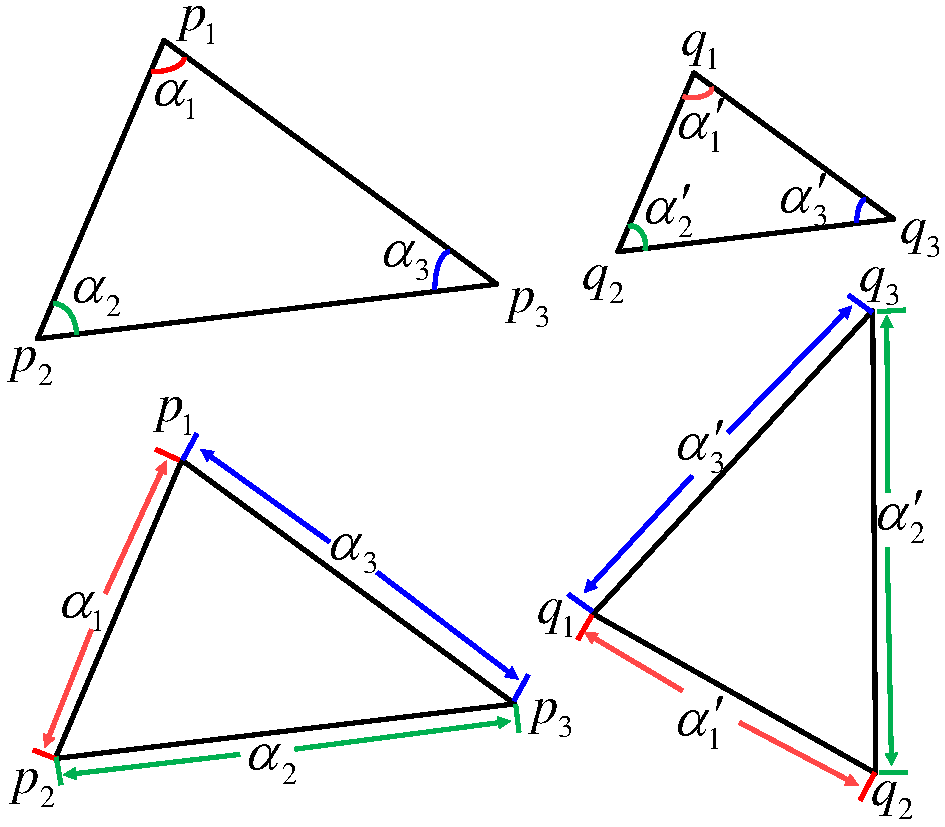
\includegraphics[width=0.8\linewidth]{figures/diagram.pdf}
  \caption{Third-order potential. The geometric constraints are: internal angle invariance in 2D (above), and edge length invariance in 3D (below).}
\label{fig:TO}
\end{figure}

%-------------------------------------------------------------------------
\subsection{Sampling strategy}
\label{subsec:sampling}

Algorithm~\ref{alg2} depends on all potential elements.
We next discuss the issue of how to sample the feature tuples to build potential items, which determines the size $|\theta_N|$ and influences matching accuracy.

For the two feature sets $P$ and $Q$,
a potential element may be obtained by using two feature tuples sampled from each feature set separately.
For $N$th-order matching, a naive way to construct the potential elements is as follows:
first find all feature tuples for $P$ and $Q$, as $F_1$ and $F_2$; then $\forall (f_{i_1}^1, f_{i_2}^1, \cdots, f_{i_N}^1)\in F_1$,
calculating the potentials for $(f_{i_1}^1, f_{i_2}^1, \cdots, f_{i_N}^1)$ with all feature tuples in $F_2$.
This naive method is very expensive, which is why sampling is used.
%%%RRM You need to say a little more about why sampling works.
%%%RRM It is not obvious that choosing just a few samples will give useful results.
We employ random sampling for general feature matching problems, but this does not preclude more directed sampling if prior knowledge of the matching problems gives
guidance.

Our sampling approach is to repeatedly randomly sample $t_1$ feature tuples from $P$, and fully sample $Q$ to find all $N_2^N$ feature tuples.
%%%RRM That is infeasible. N = N1 N2. Suppose N1 = N2 = 100.
%%%RRM Then N2 = 100^(10000) which is completely impossible.
%%%RRM Something is wrong here.
%%%RRM
%%%RRM I think the problem is here you use N here to mean the order of the matching.
%%%RRM This needs to be a different symbol, say O for order, than the N used before.
%%%RRM
For $P$, in order to cover all features in $P$ as $F_1$, we repeatedly take one feature as a required element,
and then randomly choose $t_1$ feature tuples containing this required element.
We repeat this process until all features in $P$ have been chosen once as a required element.
Then, $\forall (f_{i_1}^1, f_{i_2}^1, \cdots, f_{i_N}^1)\in F_1$, we find the $k$ most similar features in $F_2$ to build $k$ potential elements as $\phi_i^k$.
Combining all the potential elements obtained, we form the desired potential element set $\theta_N = \{\phi_i^k\}_{i=1}^{N_1 t_1}$, of size $|\theta_N| = N_1 t_1 k$.
For $P$, the sampling cost is $O(N_1\, t_1\,  k\log N_1)$.
%%%RRM I dont understand where the log comes from. You did not describe
%%%RRM anything that will obviously give log behaviour
The parameters $t_1$ and $k$ must be chosen according to the size of the feature sets.
In practice, for two feature sets each with hundreds points,
we may take $t_1 \approx 100$ and $k \approx 300$ for third- and fourth-order matching.
Our experiments demonstrate that this sampling approach works well.


The most important part of our sampling approach is to use the supersymmetry of the affinity tensor. Potential elements whose indices are permutations of each other
have the same value, so should not be repeatedly sampled.
Thus, we use a sampling constraint that the sets of feature tuples $F_1$ obtained from the sampling process should have no repetition, in the sense that
\begin{eqnarray}
\label{equ:noredun2}
\forall (f_{i_1}^1,f_{i_2}^1,\cdots,f_{i_N}^1),(f_{j_1}^1,f_{j_2}^1,\cdots,f_{j_N}^1) \in F_1,\nonumber\\ (f_{i_1}^1,f_{i_2}^1,\cdots,f_{i_N}^1)\neq\Omega(f_{j_1}^1,f_{j_2}^1,\cdots,f_{j_N}^1)
\end{eqnarray}
where $\Omega$ is an arbitrary permutation.

Earlier work~\cite{Duchenne09,Zass08} adopted random sampling,
but failed to impose any constraint on the sampling process,
leading to the possibility that feature tuples may be sampled multiple times.
For example, for third-order matching, it is possible that a feature tuple $(f_{i_1}^1, f_{i_2}^1, f_{i_3}^1)$ may be sampled from $P$ and $(f_{i_1}^2, f_{i_2}^2, f_{i_3}^2)$ from $Q$, 
and also a feature tuple $(f_{i_1}^1, f_{i_3}^1, f_{i_2}^1)$ sampled from $P$ and $(f_{i_1}^2, f_{i_3}^2, f_{i_2}^2)$ from $Q$. That will create two tensor elements $\phi_3(s_{i_1}, s_{i_2}, s_{i_3})$ with index $(s_{i_1}, s_{i_2}, s_{i_3})$ and $\phi_3(s_{i_1}, s_{i_3}, s_{i_2})$ with index $(s_{i_1}, s_{i_3}, s_{i_2})$, which are the same. However, we just need one tensor element to express the affinity measure on the assignment group $(s_{i_1}, s_{i_2}, s_{i_3})$ for any permutation of indices.
This extra sampling is not only inefficient, but may also reduce the accuracy of the power iteration: one set of symmetrically related elements  may be represented by a different number of samples than another set of  symmetrically related elements, which unbalances the power iteration process, and can lead to inaccurate results.
Therefore, our sampling method reduces the sampling cost, while also improving the accuracy of the power iteration.
